\documentclass[conference,10pt,twocolumn]{IEEEtran}
\IEEEoverridecommandlockouts
\usepackage{amsfonts}
\usepackage{amsmath,amssymb}
\usepackage{acronym}  % make an acronym
\usepackage{algorithm}
\usepackage{algorithmic}
\usepackage{balance}
\usepackage{bm}
\usepackage{bbm}
\usepackage{booktabs}
\usepackage{color, soul}
\usepackage{cite}
\usepackage{flushend}
\usepackage{graphicx}
\usepackage{indentfirst}
\usepackage{setspace}
\usepackage{tikz}
\usetikzlibrary{arrows}
\usepackage{subfigure}
\usepackage[amsmath,thmmarks]{ntheorem}
\usepackage{theorem}
% Enable Hyper-references.
\usepackage{hyperref}
\hypersetup{hidelinks, 
colorlinks=true,
allcolors=black,
pdfstartview=Fit,
breaklinks=true}

\newtheorem{theorem}{\bf Theorem}
\newtheorem{proposition}{\bf Proposition}
\newtheorem{lemma}{\bf Lemma}
\newtheorem{definition}{Definition}
\newtheorem{remark}{\bf Remark}

\theoremheaderfont{~~~\it}\theorembodyfont{\upshape}%
\theoremstyle{nonumberplain}
\theoremseparator{}
\theoremsymbol{\rule{1ex}{1ex}}
\newtheorem{proof}{Proof:}
\acrodef{SNR}[SNR]{signal-to-noise ratio}
\acrodef{DoF}[DoF]{degree of freedom}
\acrodef{FPGA}[FPGA]{field programmable gate array}
\acrodef{RF}[RF]{radio-frequency}
\acrodef{BS}[BS]{base station}
%\acrodef{RIS}[RIS]{reconfigurable intelligent surface}
%do not use \ac{RIS}
\acrodef{DL}[DL]{downlink}
\acrodef{TA}[TA]{transmit antenna}
\acrodef{RA}[RA]{receive antenna}
\acrodef{LOS}[LOS]{line-of-sight}
\acrodef{NLOS}[NLOS]{none-line-of-sight}
\acrodef{RC}[RC]{receiver combining}
\acrodef{AWGN}[AWGN]{additive white Gaussian noise}
\acrodef{DFT}[DFT]{discrete Fourier transform}
\acrodef{IRF}[IRF]{interference random field}
\acrodef{MISO}[MISO]{multiple-input single-output}
\acrodef{CSI}[CSI]{channel state information}
\acrodef{CRLB}[CRLB]{Cram{\'e}r-Rao lower bound}
\acrodef{UPA}[UPA]{uniform planar array}

\def \H {^H}
\def \opt {^{\text{opt}}}
\def \v {\bm v}
\def \w {\bm w}
\def \g {\bm g}
\def \f {\bm f}
\def \T {\bm \Theta}
\def \t {\bm \theta}
\def \x {\bm \xi}
\def \Pmax {P_{\text{max}}}
\def \ml {multi-layer }
\def \tb {transmit beamformer }
\def \sl {single-layer }
\def \diag {\text{diag}}
\def \opt {^{\text{opt}}}
\def \exp {\text{exp}}
\def \arg {\text{arg}}
\def \CN {\mathcal{CN}}
\def \VM {\mathcal{VM}}
\def \re {\text{Re}}
\def \nc {\mathcal{NC}}
\def \ch {\textcolor{red}{(cite here) }}

\newcommand{\RNum}[1]{\uppercase\expandafter{\romannumeral #1\relax}}
\renewcommand{\algorithmicrequire}{\textbf{Input:}}   %Use Input in the format of Algorithm
\renewcommand{\algorithmicensure}{\textbf{Output:}}  %UseOutput in the format of Algorithm
\newcommand{\myincludegraphics}[2][width=8.5cm]{\includegraphics[#1]{#2}}
% 12cm for onecolumn,

\ifCLASSINFOpdf
\else
\fi
\hyphenation{op-tical net-works semi-conduc-tor}
\begin{document}
\title{Interference Random Field-Based CSI Acquisition for RIS-Aided Wireless Communications}
\author{\IEEEauthorblockN{Jieao~Zhu$^*$, Kunzan~Liu$^*$, Zhongzhichao~Wan$^*$, Linglong~Dai$^*$, Tie Jun Cui$^\dagger$, and H.~Vincent~Poor$^\ddagger$}\\
\IEEEauthorblockA{ 
    $^*$Beijing National Research Center for Information Science and Technology (BNRist), \\Department of Electronic Engineering, Tsinghua University, Beijing 100084, China \\
    $^\dagger$ State Key Laboratory of Millimeter Waves, Southeast University, Nanjing 210096, China \\
    $^\ddagger$ Department of Electrical and Computer Engineering, Princeton University, NJ 08544, USA \\
    E-mails: \{zja21, lkz18, wzzc20\}@mails.tsinghua.edu.cn, tjcui@seu.edu.cn, poor@princeton.edu
}
% \thanks{J. Zhu, K. Liu, Z. Wan, and L. Dai are with the Beijing National Research Center for Information Science and Technology (BNRist) as well as the Department of Electronic Engineering, Tsinghua University, Beijing 100084, China (e-mails: \{zja21, lkz18, wzzc20\}@mails.tsinghua.edu.cn, daill@tsinghua.edu.cn).

% T. J. Cui is with the State Key Laboratory of Millimeter Waves, Southeast University, China (e-mail: tjcui@seu.edu.cn).

% H. V. Poor is with the Department of Electrical and Computer Engineering, Princeton University, USA (e-mail: poor@princeton.edu).

% This work was supported in part by the National Key Research and Development Program of China (Grant No.2020YFB1807201), in part by the National Natural Science Foundation of China (Grant No. 62031019), and in part by the European Commission through the H2020-MSCA-ITN META WIRELESS Research Project (Grant No. 956256).}
}

\maketitle

\begin{abstract}
Reconfigurable intelligent surfaces (RISs) are envisioned as a potentially transformative technology for future wireless communications.
However, RIS's inability to process signals and their attendant increased channel dimension have brought new challenges to RIS-assisted systems, which greatly increases the pilot overhead required for channel estimation.
In this paper, we propose a dimension-independent channel state information (CSI) acquisition approach in which the required pilot overhead is independent of the number of RIS elements.
In order to achieve this dimension-independent property, we propose a novel signaling method in which signals are transmitted from the base station (BS) and the user simultaneously during CSI acquisition.
Under this method, an electromagnetic interference random field (IRF) will be induced on the RIS, and we employ a sensing RIS to capture its features.
Moreover, we develop three algorithms for parameter estimation in this system, and also derive the Cram{\'e}r-Rao lower bound (CRLB) and an asymptotic expression for it. 
Simulation results verify that our proposed signal transmission method and the corresponding algorithms can achieve dimension-independent CSI acquisition for beamforming.
\end{abstract}

\begin{IEEEkeywords}
Reconfigurable intelligent surface (RIS), channel estimation, interference random field (IRF), dimension-independent CSI acquisition. 
\end{IEEEkeywords}

\section{Introduction}
Reconfigurable intelligent surfaces (RISs) are considered to be a potentially important technology for future wireless communications.
The characteristics of low cost and power consumption make RISs a promising solution for overcoming blockages, improving capacity, and reducing transmit power \cite{basar2019wireless,liu2021compact,wu2019intelligent}.
Specifically, an RIS is a large-scale array composed of passive elements, which can achieve significant beamforming gain by appropriately imposing phase shifts on the incident electromagnetic waves \cite{di2020smart}.
To achieve this beamforming gain, accurate \ac{CSI} should be acquired beforehand, which makes channel estimation an essential problem for RIS-assisted communications \cite{wei2021channel}.

Although channel estimation has been well investigated in conventional communication systems, the additional employment of RISs brings about two challenges.
Firstly, in contrast to traditional antenna array capable of transmitting, receiving, and processing the signals, RISs can only passively reflect the incident signals.
Secondly, since the number of RIS elements is usually large, the dimensions of the channels increase sharply compared with conventional communication systems, which results in unacceptably high pilot overhead for channel estimation.
These two main challenges result in the need for new channel estimation techniques for beamforming in RIS-assisted communications.

To tackle the challenges in channel estimation for RIS-assisted communications, some solutions have been proposed, which can be generally divided into two categories.
The first category modifies the hardware architecture of the RIS, which enables some signal processing capability.
For example, by sparsely replacing some of the RIS elements with active sensors capable of baseband processing, the authors of \cite{taha2021enabling} proposed a compressive sensing and deep learning-based channel estimation scheme with negligible pilot overhead. 
To further reduce the number of active sensors, in \cite{alexandropoulos2020hardware} the authors proposed an alternating direction method-based channel estimation procedure with a single \ac{RF} chain, with the help of an extended analog combiner.
The second category preserves the original hardware architecture of RISs, while conceiving new algorithms to exploit the specific features that RISs bring about.
Exploiting the two-timescale channel property in the RIS-assisted system, the authors of \cite{Huchen} proposed a two-timescale channel estimation algorithm that reduces the pilot overhead in the time-averaged sense.
In \cite{wang2020compressed}, compressive sensing-based algorithms are developed with reduced pilot overhead by exploiting the sparsity of channels in the angular domain.

Note that, in order to achieve high beamforming gain, all the above channel estimation methods are designed to estimate the full channel matrix as accurately as possible. 
However, since the channel matrix is at least of size $\mathcal{O}(N)$, where $N$ denotes the number of RIS elements, the required pilot overhead for channel estimation is usually proportional to the number of RIS elements \cite{taha2021enabling,alexandropoulos2020hardware,vlachos2019wideband,nguyen2021hybrid,Huchen,wang2020compressed,wang2020channel,kundu2021channel} in practical systems, which makes most of the existing channel estimation schemes dimension-dependent. 
This is unacceptable especially when the RIS is fabricated with a large number of elements (e.g. 2304 elements in \cite{yangfan2020coding}). 
Therefore, the following question naturally arises: {\it Does there exist a dimension-independent approach where the required pilot overhead is independent of the number of RIS elements?}

We point out that the main drawback of conventional channel estimation methods is that they only extract the mathematical features of channels, while neglecting their electromagnetic nature. 
In this paper, we first reveal that phase information about the channel can also be gathered from the phenomenon of electromagnetic interference that occurs on RISs, which we name the \ac{IRF}. To induce the \ac{IRF} on an RIS, we propose a novel pilot transmission method called simultaneous rotational signaling.
To exploit this \ac{IRF} for CSI acquisition, we employ a sensing RIS that integrates power detectors into the RIS elements to capture the features of the \ac{IRF}. Each of the power detectors can acquire its phase information independently from the \ac{IRF}, so that the required pilot overhead is independent of the number of RIS elements. 
Moreover, we develop algorithms and derive the \ac{CRLB} for the phase estimation based on the detected power detector to perform beamforming.
Numerical results verify that our developed algorithms are close to the \ac{CRLB}, and our \ac{IRF}-based methods can realize dimension-independent CSI acquisition for beamforming, while achieving near-optimal spectral efficiency. 

\textit{Notation:}
$\{L\}$ represents the set of integers $\{0,1,\cdots,L-1\}$; 
$\text{diag}(\cdot )$ is the diagonal operation;
$\mathcal{CN}\left(\mu, \sigma^2 \right)$ represents the complex univariate Gaussian distribution with the mean $\mu$ and the variance $\sigma^2$;
$\VM(\mu, \kappa)$ denotes the von Mises distribution with circular mean $\mu\in [0,2\pi]$ and centrality $\kappa$;
$\nc_{\chi_k^2}(\lambda, \sigma^2)$ is the degree-$k$ non-central chi-squared distribution with non-centrality parameter $\lambda$ and variance parameter $\sigma^2$. 
$x_{\rm BB}(t)$ denotes the baseband representation of a passband signal $x(t)$;
$I_\nu(z)$ is the $\nu$-th order modified Bessel function of the first kind. 


\section{System Model}  \label{System Model}
    In this section, we will first specify the system model of the RIS-assisted \ac{MISO} system in Subsection~\ref{RIS-assisted MISO system}. 
    Then, we will introduce traditional approaches for the corresponding beamforming design in Subsection~\ref{Beamforming}.

\subsection{RIS-assisted MISO system}\label{RIS-assisted MISO system}
    Let us consider an RIS-aided MISO system, where an $N$-element RIS is employed for enhancing the transmission from an $M$-antenna \ac{BS} to a single-antenna user. 
    Assume furthermore that the phase-shift of each element of the RIS can be continuously and independently controlled \cite{wu2019intelligent}. Then, the RIS precoding matrix can be represented by $\bm \Theta = \diag \left(\bm \theta\right )=\diag \left(\left[\theta_{1},\cdots ,\theta_{N}\right]^{T}\right)$,
    where $\theta_n (n\in \{N\})$ denotes the phase-shift of the $n$-th RIS element, satisfying $\lvert \theta_n\rvert=1$. Therefore, the signal received by the user can be written as 
    \begin{equation}
        \label{Signal model}
        y=\bm f^{H} \bm\Theta \bm G \bm w s+z,
    \end{equation}
    where $\bm f\in \mathbb C ^{N\times 1}$ and $\bm G \in \mathbb C^{N\times M}$ denote the channel from the RIS to the user and the channel from the BS to the RIS, respectively; $\bm w\in \mathbb C^{M\times 1}$ denotes the beamforming vector at the transmitter BS, with power constraint $\left\Vert \bm w\right \Vert_{2}^{2}\leq P_{\text{max}}$; $s$ denotes the normalized BS transmitted symbol; $z\sim \mathcal{CN}\left(0,\sigma_{z}^{2}\right)$ denotes the \ac{AWGN}. To focus on RIS beamforming, direct links are neglected in this paper. 

\subsection{Beamforming} 
    \label{Beamforming}
    In this paper, we assume that the locations of the \ac{BS} and the RIS are unchanged, which can provide us a beamforming approach expressed as
    \begin{equation}
        \label{traditional beamforming}
        \bm w=\sqrt{P_{\rm max}}\bm a\left(\alpha\right),\quad \theta_{n} = \exp\left(-{\rm j} \arg\left(f_{n}^{*}\bm g_{n}^{T}\bm w\right)\right),~\forall n\in \{N\},
    \end{equation}
    where $\bm a(\alpha)$ denotes the array steering vector with respect to the wave departure angle $\alpha$ of the BS antenna array, and $\bm G = \left[\bm g_{1}, \cdots, \bm g_{N}\right]^{T}$. Note that the optimal RIS phase is only determined by $\arg\left(f_{n}^{*}\bm g_{n}^{T}\bm w\right)$, i.e., the phase difference between the BS-RIS channel $\bm g_n^T$ and the user-RIS channel $f_n^*$. 

% \section{Interference Random Field}
% \label{Interference Random Field}
%     In this section, the signal model for the \ac{IRF} will be first introduced in Subsection~\ref{Models for IRFs}. Then, in order to acquire the CSI, the simultaneous rotational signaling method will be proposed in Subsection~\ref{Simultaneous Rotational Signaling and Interference Detection}. 

\subsection{Signal Model for IRF}
\label{Models for IRFs}
    Suppose two signals impinge upon the RIS simultaneously, creating an interference field at the $n$-th RIS element. Denote the symbol transmitted from the \ac{BS} by $s$, and the symbol transmitted from the user by $s'$. In order to perform channel estimation by exploiting the \ac{IRF}, we need to probe the interference fringes, i.e., the power of the \ac{IRF}. Following the notations in Section~\ref{System Model}, we obtain the noisy IRF signal by adding up the two impinging baseband signals
    \begin{equation}
        \begin{aligned}
            E_{{\rm BB, IRF}}(t) &= E_{{\rm BB, BS}}(t)+E_{{\rm BB,user}}(t)+v(t)\\
            &=\bm g_{n}^{T}\bm w s+f_{n}^{*} w' s' +v(t),
        \end{aligned}
    \end{equation}
    where $v(t)\sim \mathcal{CN}(0,\sigma_{v}^{2})$ is the electromagnetic noise signal, $\bm w$ and $w'$ are the beamforming vector at the BS side and the user side satisfying $\Vert \bm w \Vert_{2}^{2}\leq P_{\text{max}}$ and $|w'|^{2}\leq P'_{\text{max}}$, respectively,
    $s$ is the symbol transmitted from the BS to RIS, and $s'=e^{{\rm j} \psi(t)}$ is the time-varying transmitted symbol from the user to the RIS.  
    Since the interference fringes are not sensitive to a global phase change, we can safely assume that $s=1$, and then the relative phase between the user and the BS can be fully characterized by a time-varying phase function $\psi(t)$.  

    Furthermore, by defining $\alpha = \left\vert\bm g_{n}^{T}\bm w\right\vert$, $\beta = \left\vert f_{n}^{*} w' \right\vert$, and the phase difference between the \ac{BS}-RIS link\footnote{Since it is usually difficult to obtain the optimal BS beamforming vector $\bm w$, during the CSI acquisition procedure, we fix $\bm w$ to a steering vector that guides most of the signal energy to the RIS aperture. As a result, $\bm g_n^T \bm w$ can be treated as the equivalent link seen by the symbol $s$.} and the RIS-user channel as $\varphi = \arg\left(f_{n}^{*}w'\right)-\arg\left(\bm g_{n}^{T}\bm w\right)$, then the power of the \ac{IRF} can be written as
    \begin{equation}
        \label{eqn:power of interference}
        \begin{aligned}
            P(t)&=A \left| E_{{\rm BB, IRF}} (t)\right |^{2}+\zeta\\
            &=\underbrace{A\left[\alpha^{2}+\beta^{2}+2\alpha\beta\cos\left(\psi(t)+\varphi\right)\right]}_{\text{IRF power signal}}+\\
            & \underbrace{2A\Re\left\{\left(\alpha+\beta e^{{\rm j}\left(\psi(t)+\varphi\right)}\right)v'^{*}(t)\right\}+A\left|v'(t)\right|^{2}+\zeta}_{\text{Noise}},\\
        \end{aligned}
    \end{equation}
    where $\zeta$ is the noise introduced by digital signal processing after measuring the IRF power, $A$ is the amplification factor of the power sensor, and the equivalent electromagnetic noise $v'(t) = e^{{\rm j}{\rm arg}({\bm g}_n^T \bm w)}v^*(t)$ obeys the same distribution as $v(t)$ for any time $t$.
    The name IRF comes from the randomness of the unknown $\varphi$, the unknown noise realization, and the interferential nature of the field.

    The phase difference $\varphi$ defined here will play an important role in our following channel estimation, since it carries enough CSI for beamforming, which will be justified in the next section. To estimate the phase difference $\varphi$, we need enough observations from the sensor-detected power signal $P(t)$. For simplicity and without loss of generality, we can assume $\psi(t)=\frac{2\pi}{T_{s}} t$, where $T_s$ is the symbol period. Furthermore, assume that $L$ observations $P[l]=P(t_{l})$ located at equally-spaced instants $t_{l}=\frac{l}{L}T_{s}$ for all $l\in \{L\}$
    are used for estimation of the phase difference $\varphi$.




\section{Sensing RIS-Based Channel Estimation}
\label{Sensing RIS-Based Channel Estimation}
In this section, we will first briefly introduce the hardware architecture required for detecting the \ac{IRF} in Subsection~\ref{Hardware Architecture of Sensing RIS}. 
Then, the signaling procedure for creating an \ac{IRF} will be introduced in Subsection~\ref{Simultaneous Rotational Signaling and Interference Detection}.
The core concept of IRF channel estimation and beamforming procedures will be introduced in Subsection~\ref{IRF Channel Estimation and Beamforming}. 
Finally, Subsection~\ref{Pilot Overhead} will include the analysis on pilot overhead and computational complexity of our proposed IRF-based CSI acquisition methods. 

\subsection{Hardware Architecture of Sensing RIS} \label{Hardware Architecture of Sensing RIS}

    \begin{figure}[!t]
        \centering
        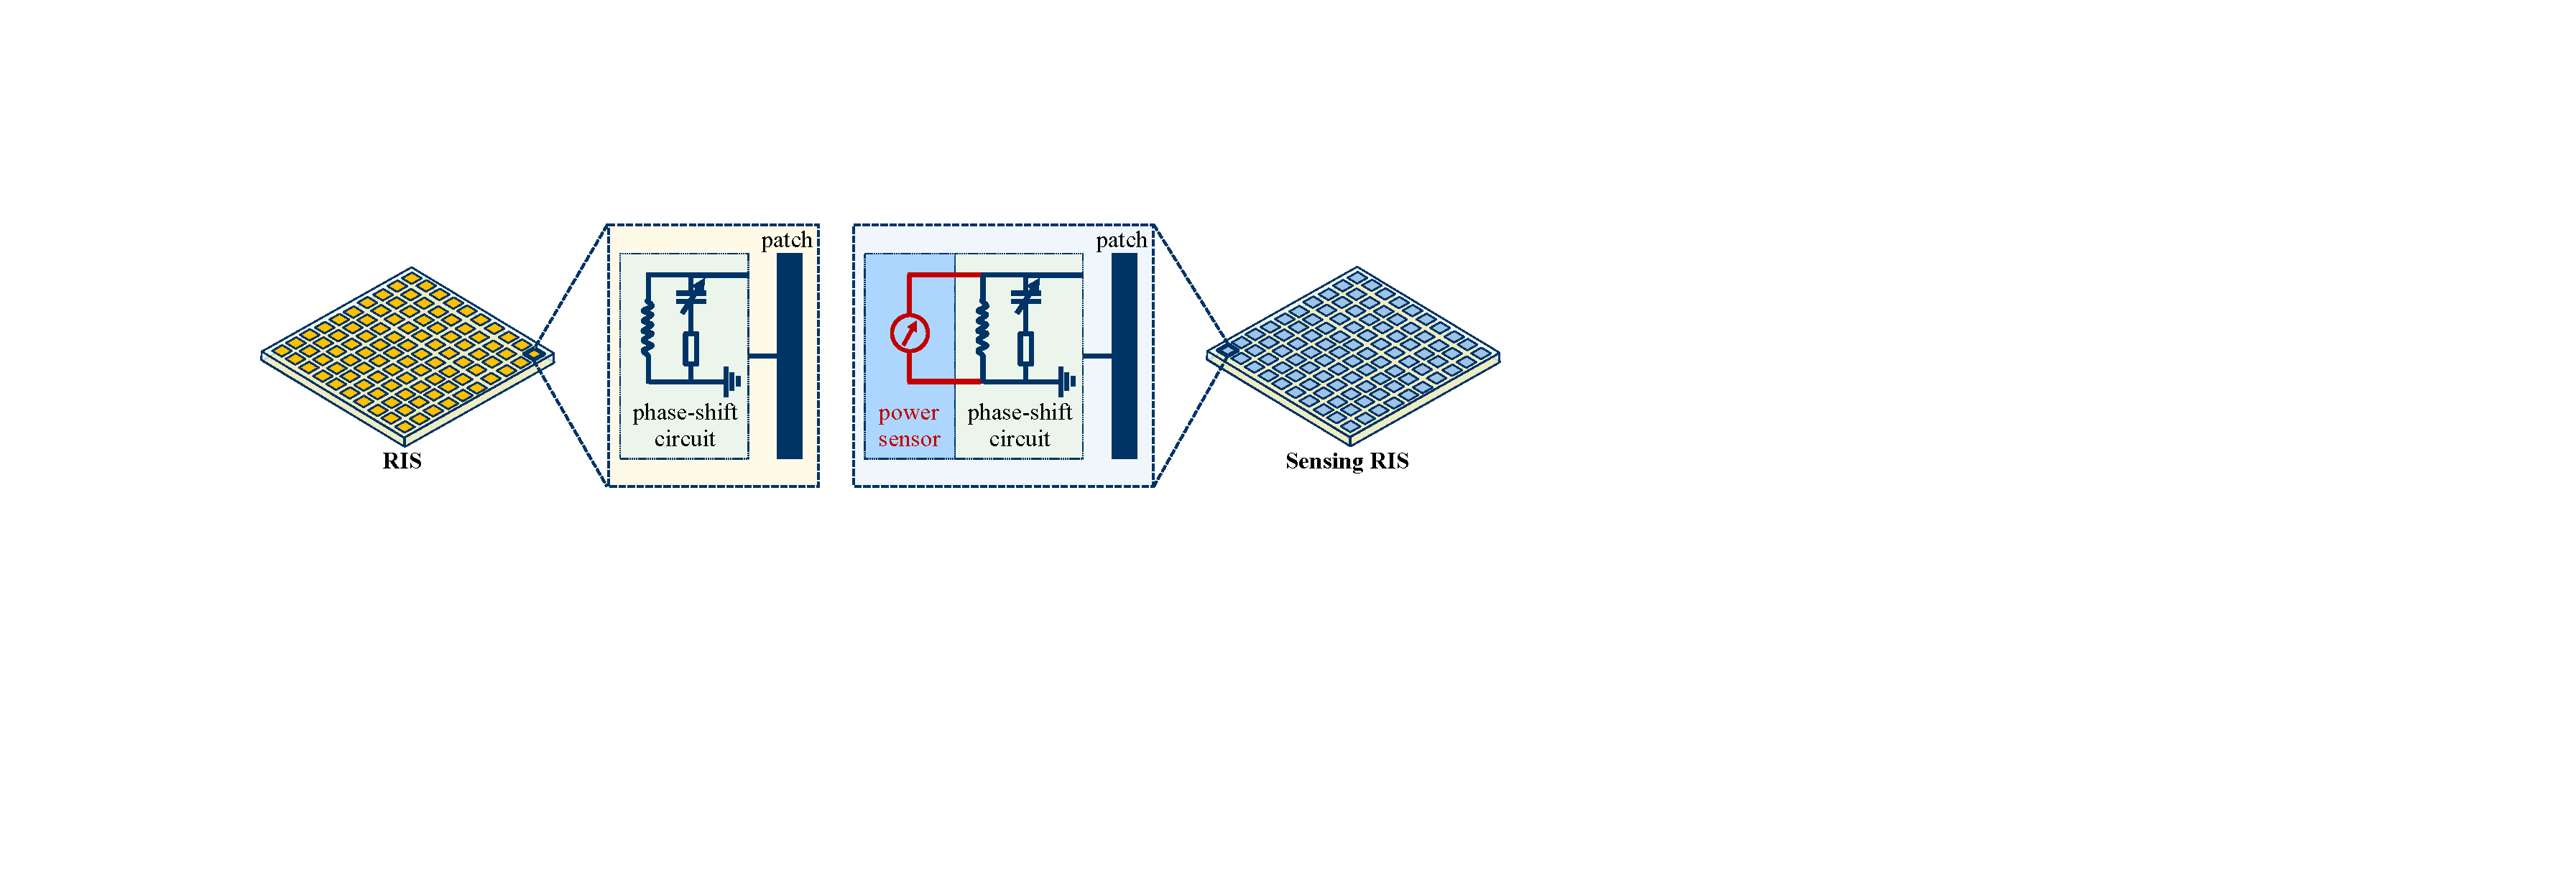
\includegraphics[width=.45\textwidth]{figures/hardware.pdf}
        \centerline{(a)~~~~~~~~~~~~~~~~~~~~~~~~~~~~~~~~~~~~~~~~~~~~~~(b)}
        \caption{Comparison of hardware architectures. (a) Traditional RIS. (b) Proposed sensing RIS.}
        \label{fig:hardware}
    \end{figure}
    
To obtain the amplitude of the induced \ac{IRF}, inspired by the sensing metasurface \cite{ma2019smart}, we propose a hardware architecture named sensing RIS.
In contrast to traditional RIS architecture shown in Fig.~\ref{fig:hardware}~(a), where each RIS element includes a phase-shift circuit and a patch antenna, each sensing RIS element additionally integrates a power sensor which is responsible for detecting the amplitude of the IRF \cite{ma2020smartsensing}, as shown in Fig.~\ref{fig:hardware}~(b).
Since all of the RIS elements can sense and adjust the phase independently from one another, low-cost microcontroller units (MCUs) can be attached locally to each RIS element to allow parallel computation of the optimal phases. 
However, for extremely large-scale RIS systems, sparse sensing and controlling may be preferred to reduce cost and hardware complexity. 

\subsection{Simultaneous Rotational Signaling and Interference Detection} \label{Simultaneous Rotational Signaling and Interference Detection}
    \begin{figure}[!t]
        \centering
        \includegraphics[width=.45\textwidth]{data/protocol.pdf}
        \caption{Simultaneous rotational signaling scheme. The IRF power is the instantaneous total power of the BS-RIS signal and the user-RIS signal. The composite power waveform that appears on RIS enables our algorithm to obtain the desired CSI. The parameters $\alpha$ and $\beta$ are estimated from the signals $P_{\alpha}(t), P_{\beta}(t)$ measured during the first two time slots, and $\varphi$ is estimated by IRF signal $P(t)$ that occurs during the third time slot.}
        \label{fig:protocol}
    \end{figure}

    Interference allows noncoherent power sensors to perform coherent detection. 
    To clarify this, let us consider the $n$-th RIS element. If the BS transmit a fixed symbol $s=1$ while the user transmits a rotational symbol $s'=e^{{\rm j}\psi(t)}$, then the detected IRF power on the $n$-th element will vary over time. 
    Thus, the desired CSI can be drawn from the varying IRF power signal received by the $n$-th element, as is shown in Fig.~\ref{fig:protocol}. 

    \begin{figure}[!t]
        \centering
        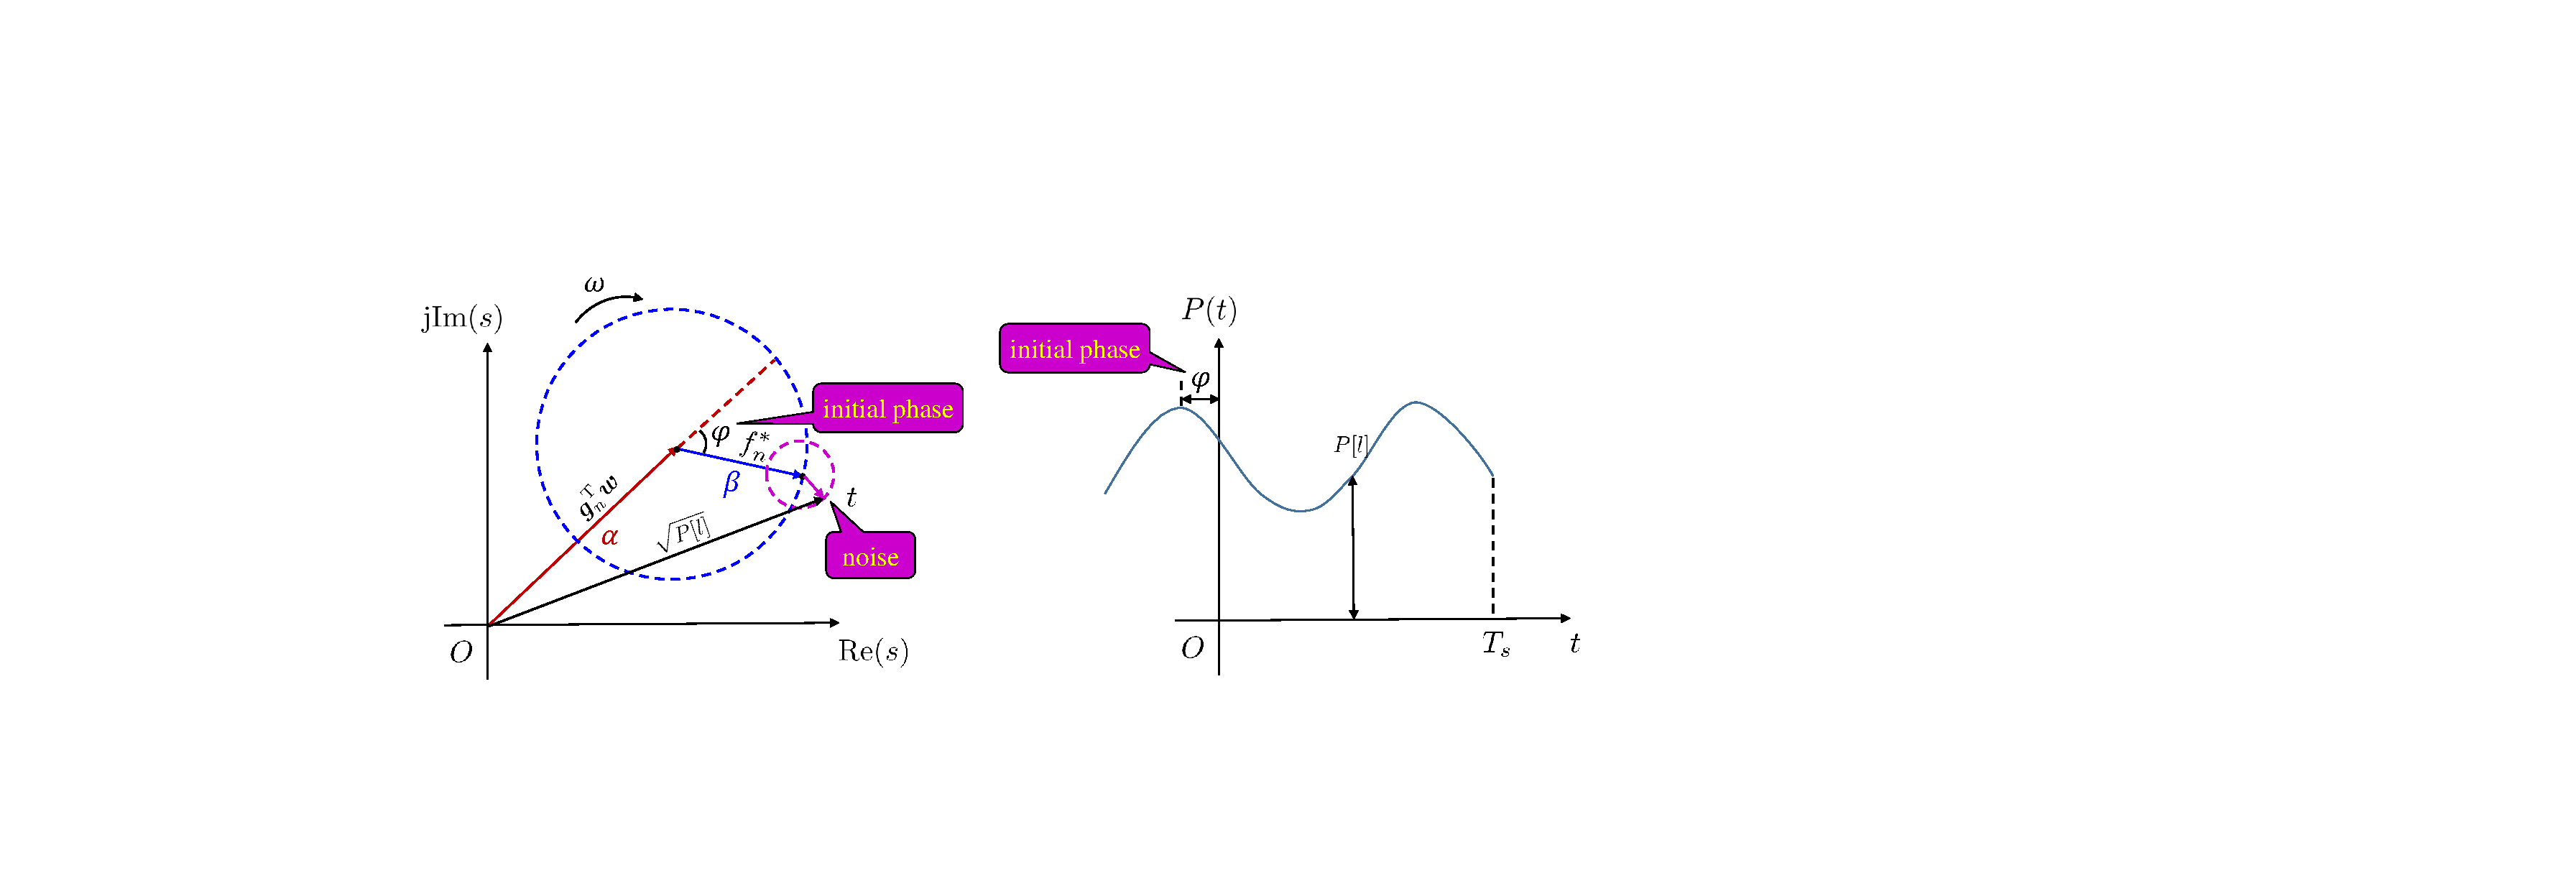
\includegraphics[width=.45\textwidth]{figures/phasor.pdf}
        \caption{Phasor representation of the \ac{IRF} on each RIS element. Red vector represents the complex BS-RIS signal ${\bm g}_n^T{\bm w}$; Blue vector represents the complex user-RIS signal $f_n^*w'$; $\alpha$ and $\beta$ denote the amplitude of these signals respectively. In our signaling method, the BS transmits a fixed symbol $s=1$, while the user transmits a rotating symbol $s'=e^{{\rm j}\psi(t)}$, causing the output of the power sensor $P(t)$ to vary in a waveform that is similar to a sine curve.}
        \label{fig:phasor}
    \end{figure}
    To further analyze the interference, we focus on the received IRF signal $P(t)$ of the $n$-th RIS element. 
    Note that the power of interference field measured at instant $t$, expressed by \eqref{eqn:power of interference}, exhibits a sinusoidal waveform, as is shown in Fig.~\ref{fig:phasor}. 
    The initial phase ($t=0$) of this sinusoidal waveform is uniquely determined by $\varphi$.
    Thus, if we have access to the power received by the $n$-th element at successive instants $t_l$, it is possible to retrieve the phase difference $\varphi$. 
    However, according to \eqref{traditional beamforming}, it is the phase sum of the RIS-user channel and the BS-RIS channel, i.e., $\arg({\bm g}_n^{T}{\bm w})+\arg(f_n^*w')$, that determines the optimal phase-shift of the $n$-th element. Given the phase difference $\varphi = \arg\left(f_{n}^{*}w'\right)-\arg\left(\bm g_{n}^{T}\bm w\right)$, in order to acquire the phase sum, we have to assume that the phase $\arg({\bm g}_n^{T}{\bm w})$ is known in advance. 
    This assumption is reasonable, because the BS-RIS link often exhibits a quasi-static property \cite{Huchen}, and can be calculated from the geometry, i.e., the locations of the BS and the RIS. 

\subsection{IRF Channel Estimation and Beamforming} \label{IRF Channel Estimation and Beamforming}
    The \ac{IRF} channel estimation and beamforming procedure can be divided into three steps:
    \begin{enumerate}
        \item Simultaneous rotational signaling and power sensing; 
        \item Phase estimation based on power data;
        \item Integrate phase information and other CSI to perform beamforming. 
    \end{enumerate} 
    For the sake of clarity, we present the complete IRF-based RIS beamforming procedure by pseudo codes, which is shown in {\bf Algorithm~\ref{alg:IRF-Beamforming}}:
    \begin{algorithm}[H] 
        \caption{Near-optimal RIS Beamforming by IRF} \label{alg:IRF-Beamforming}
        \setstretch{1.1}
        \begin{algorithmic}[1]
            \REQUIRE Number of RIS elements $N$, IRF power signals detected on each RIS element $P_{\alpha}(t), P_{\beta}(t)$ and $P(t)$.
            \ENSURE RIS phase-shift matrix ${\bm \Theta}$.
            \FOR{$n=1,2,\cdots,N$}
                \STATE Estimate $\alpha$ and $\beta$ from $P_{\alpha}(t)$ and $P_{\beta}(t)$.
                \STATE Estimate phase difference $\varphi_n$ from $P(t)$, $\alpha$ and $\beta$. 
                \STATE Estimate $\psi_{n} = {\rm arg}(\bm g_{n}^{T}\bm w)$ from known locations of BS and RIS
                \STATE $\theta_n \leftarrow \exp(-{\rm j}(\varphi_n + 2\psi_n))$
            \ENDFOR
            \STATE ${\bm \Theta} \leftarrow \diag\left(\left[\theta_1, \theta_2, \cdots, \theta_N\right]^{T}\right)$
            \RETURN ${\bm \Theta}$
        \end{algorithmic}
    \end{algorithm}

\subsection{Pilot Overhead and Computational Complexity}\label{Pilot Overhead}
    In our proposed IRF-based CSI acquisition method, the pilot overhead is reduced to $\mathcal{O}(1)$, which is independent of the RIS dimension $N$. 
    The reason is that, no matter how many RIS elements are employed, the IRF appears on them simultaneously. 
    Thus, both the channel estimation and beamforming can be fulfilled within only three pilot symbols, as is depicted in Fig.~\ref{fig:protocol}. 
    Thus, the pilot overhead is independent of the RIS dimension $N$. 
    To the best of our knowledge, this dimension-independent property is unprecedented. 
    
    \begin{table}[t]
        \caption{Pilot Overhead Comparison of Different CSI Acquisition Methods}
        \label{tab:pilot overhead comp CE}
        \centering
        \begin{tabular}{|l|r|r|}
                \hline 
                CSI acquisition method & Minimum pilot overhead\\ 
                \hline
                MVU\cite{jensen2020optimal}         & $NK+K$     \\
                \hline
                Multi-user\cite{wang2020channel}  & $K+N+ \lceil \frac{(K-1)N}{M} \rceil$\\
                \hline
                CS\cite{wei2021channel}          & $\mathcal{O}(KS\log N)$ \\
                \hline 
                Two-timescale\cite{Huchen} & $\frac{2(N+1)}{\alpha} + K\lceil N/M\rceil +K$  \\
                \hline 
                Proposed IRF & 3 \\ 
                \hline
        \end{tabular}
    \end{table}

    Table~\ref{tab:pilot overhead comp CE} compares the pilot overhead of our proposed IRF method with other different CSI acquisition methods. Our IRF method needs exactly 3 pilot slots for a single user, regardless of the number of RIS elements. 

\section{Phase Estimation Algorithms}
In this section, three phase estimation algorithms will be proposed in Subsection~\ref{DFT method}, \ref{ML method}, and \ref{von Mises-EM method} respectively, which constitute the core of the \ac{IRF} channel estimation and beamforming algorithm.

\subsection{DFT method}  \label{DFT method}
    The key challenge of the IRF channel estimation and beamforming is the phase estimation step, i.e., how to obtain the phase difference $\varphi$. Since the interferential power $P(t)$ exhibits a sinusoidal waveform, Fourier transforms can be applied to extract its phase. Apply $L$-point \ac{DFT} to the discrete-time  observed sensor detection signals $P[0],\cdots ,P[L-1]$, and we have
    \begin{equation}
        \label{DFT}
        p[l']=\sum\nolimits_{l=0}^{L-1}P[l]e^{-{\rm j}\frac{2\pi}{L}ll'},\quad \forall l'\in \{L\}.
    \end{equation}
    Specifically, we have the complex amplitude of the first harmonic $p[1]$ as 
    \begin{equation}
        \label{DFT l=1}
        p[1]=LA\alpha\beta  e^{{\rm j}\varphi}.
    \end{equation}
    Then, the phase $\varphi$ can be estimated as
    \begin{equation}
        \label{LS estimate result}
        \hat{\varphi}=\arg\left(\frac{p[1]}{LA\alpha\beta}\right) = \arg\left(p[1]\right).
    \end{equation}
    Note that this DFT method simply ignores the non-Gaussian noise. For Gaussian noise, the DFT method is optimal. However, in fact, the noise in \eqref{eqn:power of interference} contains a squared term of Gaussian noise, resulting in the noise being non-Gaussian. Thus, we further conceive an ML method, as described in the following Subsection~\ref{ML method}. 

\subsection{Newton-ML method}  \label{ML method}
    Suppose the noise field $v'(t)=v'_R(t) + {\rm j}v'_I(t)\sim \mathcal{CN}(0, \sigma_v^2)$, and the noise of the power sensor is $\zeta \sim \mathcal{N}(0, \sigma_{\zeta}^2)$. 
    Without loss of generality, we can assume that the sensor noise power $\sigma_{\zeta}^2$ is much weaker than the electromagnetic noise field $v'(t)$.
    Thus, we assume $\sigma_{\zeta}^2=0$ in the following discussion.  
    As a result, the distribution of $P(t) = A\left|E_{{\rm BB}, {\rm IRF}}(t)\right|^2$ is a non-central chi-squared distribution $\nc_{\chi_2^2}(A(\mu_{R}^2+\mu_{I}^2),  A\sigma_v^2/2)$ with degrees of freedom $k=2$, and mean values $\mu_{R}, \mu_{I}$ given by
    \begin{equation}
        \mu_{R} = \alpha + \beta \cos(\psi(t)+\varphi),\quad  \mu_{I}  = \beta \sin(\psi(t)+\varphi).
        \label{chi2 distribution mean values}
    \end{equation}
    Thus, according to \eqref{eqn:power of interference}, the output signal of the power sensor is given by 
    \begin{equation}
        P(t)  = A\left((v'_{R} + \mu_{R})^2 + (v'_{I} + \mu_{I})^2 \right)
        \label{eqn:sensor power}
    \end{equation}
    Let us define the noncentral parameter $\lambda(t)$ as
    \begin{equation}
        \lambda(t)  = A(\mu_{R}^2 + \mu_{I}^2) = A\left[\alpha^{2}+\beta^{2}+2\alpha\beta\cos\left(\psi(t)+\varphi\right)\right].
    \end{equation}
    Then, according to the definition of the $\nc_{\chi_2^2}$, the p.d.f of $P(t)$ is given by the zeroth-order modified Bessel function of the first kind 
    \begin{equation}
        f_{P}(x) = \frac{1}{A\sigma_{v}^2} \exp\left(-\frac{x+\lambda(t)}{A\sigma_v^2}\right)I_{0}\left(\frac{\sqrt{\lambda(t) x}}{A\sigma_v^2/2}\right),\quad x \geq 0.
        \label{ML single observation}
    \end{equation}
    Then, the log likelihood function of $\varphi$ based on the observations $P[l]$ can be represented by
    \begin{equation}
        \begin{aligned}
        & \mathcal{L}(\varphi) =\\
        & \sum_{l=0}^{L-1}\left[-\frac{P[l] + \lambda_l}{A\sigma_v^2} + \log I_0\left(\frac{\sqrt{P[l] \lambda_l}}{A\sigma_v^2/2}\right)\right] - L\log(A\sigma_v^2),
        \end{aligned}
        \label{ML likelihood}
    \end{equation}
    where $\lambda_l := \lambda(t_l)$. By taking the derivative and the second-order derivative of \eqref{ML likelihood}, we can perform the Newton iteration to obtain $\hat{\varphi}$, by iteratively using the updating formula
    \begin{equation}
        \hat{\varphi}^{(k+1)} = \hat{\varphi}^{(k)} - \frac{\mathcal{L}'(\hat{\varphi}^{(k)})}{\mathcal{L}''(\hat{\varphi}^{(k)})}.
        \label{eqn:Newton-ML renewal formula}
    \end{equation}
    Note that during the calculation of \eqref{eqn:Newton-ML renewal formula}, $A, \sigma_v, \alpha, \beta$ and the received signal $P[l]$ are all assumed to be known.
        % \begin{equation}
    %     R'(z)=1-R^2(z)-\frac{1}{z}R(z),
    %     \label{eqn:R function derivative property}
    % \end{equation}

\subsection{von Mises-EM method}    \label{von Mises-EM method}
    The Newton-ML algorithm is asymptotically optimal. 
    However, the computation of the Newton-ML estimator is quite complicated due to the intensive calculation of modified Bessel functions. 
    Now we introduce an iterative method for estimating $\varphi$ without any computation of such special functions.
    Our method is based on the von Mises distributions \cite{gatto2007generalized}.

    The von Mises distribution $\VM(\mu, \kappa)$ is a two-parameter distribution on $[0, 2\pi]$, with the probability density function given by 
    \begin{equation}
        p(\theta|\mu, \kappa) = \frac{\exp(\kappa \cos(\theta - \mu))}{2\pi I_0(\kappa)}, \quad 0\leq \theta \leq 2\pi,
    \end{equation}
    where $\mu \in [0,2\pi]$ and $\kappa >0$ being the cyclic location parameter and the concentration parameter. 
    Note that the von Mises distribution is a distribution on a circle, thus it acts as a perfect prior distribution of a phase estimation problem under Gaussian noise. 
    The following two lemmas: {\bf Lemma \ref{lemma_1}} and {\bf Lemma \ref{lemma_2}} reveal the interactions between the von Mises distribution and the complex Gaussian noise distribution.
    \begin{lemma}[Bayesian estimation of $\VM$]\label{lemma_1} \mbox{}\par
        Let $\theta \sim \VM(\mu, \kappa)$, and $z|\theta \sim \CN(e^{{\rm j}\theta}, \sigma^2)$. Then the posterior distribution $\theta | z$ is also a von Mises distribution $\VM(\mu', \kappa')$ with parameters $\mu'$ and $\kappa'$ satisfying $\kappa' e^{{\rm j}\mu'} = \kappa e^{{\rm j}\mu} + 2z/\sigma^2$.
    \end{lemma}
        \begin{IEEEproof}
        Please refer to the journal version of this paper. 
    \end{IEEEproof}
    
    In this paper, we also use $\VM(\kappa e^{{\rm j}\mu})$ to denote the von Mises distribution $\VM(\mu, \kappa)$. 
    This representation provides convenience for the calculation of the posterior distribution of the von Mises distribution in Bayesian inference.

    \begin{lemma}[$\VM$ and circular $\CN$]\label{lemma_2} \mbox{}\par
        Suppose $z \sim \CN(z_0, \sigma^2)$, where $z_0 \in \mathbbm{C}$, and a positive radius $r>0$. Then the posterior distribution of angle $\theta= {\rm arg} (z)$, constrained on a circle $|z|=r$ obeys the von Mises distribution
        \begin{equation}
            p(\theta |\, |z|=r) \sim \VM\left({\rm arg}(z_0), \frac{r|z_0|}{\sigma^2/2}\right).
        \end{equation}
    \end{lemma}
    \begin{IEEEproof}
        Replacing $z$ by $r e^{{\rm j} \theta}$ give rise to the conclusion immediately. 
    \end{IEEEproof}
    
    Combining the results of {\bf Lemma \ref{lemma_1}} and {\bf Lemma \ref{lemma_2}}, we can then construct the EM algorithm for estimating $\varphi$. Since the output of the power sensors $P[l]$ does not contain phase information, we can treat the phases as latent variables. Let $s_l = \sqrt{P[l]/A}$ be the noisy estimation for $|\alpha + \beta e^{{\rm j} (\varphi + \psi_l)} + v_l|$, and $\theta_l$ be the latent variables $\arg (\alpha + \beta e^{{\rm j} (\varphi + \psi_l)} + v_l)$ that are not observable. 
    Since the noise $v_l \sim {\rm i.i.d.}\;\CN(0, \sigma_v^2)$, then from {\bf Lemma \ref{lemma_2}}, $\theta_l | s_l, \varphi \sim \VM(\arg(\alpha + \beta e^{{\rm j} (\varphi + \psi_l)}), s_l |\alpha + \beta e^{{\rm j} (\varphi + \psi_l)}|/(\sigma_v^2/2))$. Thus, we can infer the latent variables by ML estimation 
    \begin{equation}
        \hat{\theta}_{l, {\rm ML}} | s_l, \varphi = \arg(\alpha + \beta e^{{\rm j} (\varphi + \psi_l)}).
        \label{eqn:E-step}
    \end{equation}
    After inferring the latent variables $\hat{\theta}_{l, {\rm ML}}$, we can update the estimation of $\varphi$ using Bayesian rule in {\bf Lemma \ref{lemma_1}}
    \begin{equation}
        \varphi | s_l, \theta_l \sim \VM\left( \kappa e^{{\rm j} \mu} + \frac{\beta}{\sigma_v^2/2}\sum_{l=0}^{L-1}{\left(s_l e^{{\rm j}\theta_l}-\alpha\right)e^{-{\rm j} \psi_l}}\right),
        \label{eqn:M-step}
    \end{equation}
    where the coefficient $\beta/(\sigma_v^2/2)$ comes from scaling the phasor in Fig.~\ref{fig:phasor} by a factor $\beta^{-1}$ and applying {\bf Lemma \ref{lemma_1}}.
    Performing E-step with \eqref{eqn:E-step} and M-step with \eqref{eqn:M-step} alternately, then the estimation precision for $\varphi$ can be iteratively improved. Note that although the modified Bessel functions appear in the density function of von Mises distribution, the bother is avoided in the von Mises-EM algorithm. The pseudo code of von Mises-EM algorithm is collected in {\bf Algorithm \ref{alg:VM-EM}}.

    \begin{algorithm}[htbp] 
        \caption{von Mises-EM phase estimation (VM-EM algorithm)} \label{alg:VM-EM}
        \setstretch{1.1}
        \begin{algorithmic}[1]
            \REQUIRE Incident wave intensity $\alpha$, $\beta$; sensor data $P[l]$; amplification factor $A$ and noise variance $\sigma_v^2$; predefined phase shifts $\psi_l=\omega t_l$.
            \ENSURE $\hat{\varphi}$
            \STATE $s_l \leftarrow \sqrt{P[l]/A}, \quad \forall l\in \{L\}$
            \STATE $\hat{\varphi} \leftarrow \arg\{{\rm FFT}(P)[1]\}$
            \STATE $\kappa \leftarrow 1$
            \WHILE {$\hat{\varphi}$ not convergence}
                \STATE $\mu_l \leftarrow \alpha + \beta e^{{\rm j} (\hat{\varphi}+\psi_l)}, \quad \forall l\in \{L\}$
                \STATE $w_l \leftarrow s_l e^{{\rm j} \arg(\mu_l)} - \alpha, \quad \forall l\in \{L\}$
                \STATE $z_\varphi \leftarrow \kappa e^{{\rm j} \hat{\varphi}} + \beta \left( \sum_{l=0}^{L-1}{w_l e^{-{\rm j} \psi_l}}\right) / (\sigma_v^2/2)$
                \STATE $\hat{\varphi} \leftarrow \arg(z_\varphi)$
                \STATE $\kappa \leftarrow |z_\varphi|$
            \ENDWHILE
            \RETURN $\hat{\varphi}$
        \end{algorithmic}
    \end{algorithm}
    
\section{Performance Analysis}
\label{Performance Analysis}
    In this section, we derive the exact expression of the CRLB in the phase estimation problem. 
    To simplify the calculation, we provide an asymptotic expression of the CRLB.

%\subsection{The CRLB} \label{The CRLB}
%    In the previous section, we have introduced three phase estimation methods. 
%    A natural question is how accurate can these phase estimators be. 
%    From \eqref{eqn:sensor power}, we can discover that the phase estimation is, in fact, a probabilistic parameter estimation problem, where the distributions of the observable variables are controlled by the parameter $\varphi$. 
%    Thus, the ``best'' mean squared error of any unbiased estimator is lower-bounded by the CRLB \cite{casella2021statistical} 
%    \begin{equation}
%        \mathbb{E}\left(\hat{\varphi}-\varphi\right)^2 \geq {\rm CRLB}(\varphi) = -\frac{1}{\mathbb{E}_{x\sim p_\varphi}\left[\frac{\partial^2}{\partial\varphi^2}\log p_{\varphi}(x)\right]},
%        \label{eqn:CRLB definition}
%    \end{equation}
%    where $p_{\varphi}(x)$ is the distribution of $x$ when the parameter is $\varphi$, and in this paper $p_{\varphi}(x)$ obeys a non-central chi-squared distribution. 
%
%    The evaluation of CRLB in non-coherent parameter estimation was first formulated in \cite{jiang2016cramer}, where the authors introduced Gaussian approximation in order to obtain a simple closed-form CRLB expression. Unfortunately, this approximation only holds for very large non-centrality parameter $\lambda$, i.e., large interferential SNR $\gamma=\lambda/A\sigma_v^2$. Thus, an exact expression of the CRLB is required in our \ac{IRF} methods. However, without Gaussian approximation techniques, fatal complexity about Bessel functions will occur, making the analysis nearly intractable. 
%
%    To overcome this difficulty, we first perform exact analysis, and then approximated asymptotic analysis. The difficulty of manipulating Bessel functions is conquered by asymptotic expansion techniques \cite{silverman1972special}. Satisfactory asymtotic results are acquired in the absence of exact closed-form expression of the CRLB. These results will be introduced in the following subsection.  
%    %In the following two subsections, {\bf Theorem \ref{thm:precise CRLB}} reveals  
    
\subsection{Exact Expression of the CRLB} \label{Precise CRLB}
In Section \ref{Sensing RIS-Based Channel Estimation}, we have introduced three phase estimation methods to solve the probabilistic parameter estimation problem.
We derive the CRLB of the estimation in \textbf{Theorem \ref{thm:precise CRLB}}.
    
    \begin{theorem}[Non-central Chi-Squared CRLB] \label{thm:precise CRLB}\mbox{}\par
        Suppose the probabilistic model is specified by \eqref{eqn:sensor power}, where $L$ observations $P[0],\cdots,P[L-1]$ are obtained. Then the CRLB of this $L$-point phase estimation problem is given by
        \begin{equation}
            \frac{1}{{\rm CRLB}(\varphi)} = K^2(\bar{\gamma})^2 \sum_{l=0}^{L-1}\sin^2(\psi_l+\varphi)\left(1/\gamma_l-g(\gamma_l)\right),
            \label{eqn:precise_CRLB}
        \end{equation}
        where $K=2\alpha\beta/(\alpha^2+\beta^2)$, $a=A\sigma_v^2$, $\gamma_l=\lambda_l/a=\left(\alpha^2+\beta^2+2\alpha\beta \cos(\psi_l+\varphi)\right)/\sigma_v^2$, and $\bar{\gamma}$ is the arithmetic mean of all the $\gamma_0,\cdots,\gamma_{L-1}$. The function $g(\gamma)$ is defined as 
        \begin{equation}
            \begin{aligned}
                g(\gamma)  = \int_{0}^{+\infty}\gamma t \, {\rm exp}(-\gamma(1+t))\, I_0\left(2\gamma\sqrt{t}\right) \times \\ 
                \left(1-R^2\left(2\gamma\sqrt{t}\right)\right){\rm d}t,
            \end{aligned}
            \label{eqn:precise_g_function}
        \end{equation}
        and $R(z)=I_1(z)/I_0(z)$. 
    \end{theorem}
    \begin{IEEEproof}
        Please refer to the journal version of this paper. 
    \end{IEEEproof}

    From \textbf{Theorem \ref{thm:precise CRLB}}, we note that the CRLB of the phase estimation problem is completely determined by the two parameters $K$ and $\bar{\gamma}$, which are the interferential contrast and the average interferential SNR, respectively. 
    However, this exact CRLB expression is difficult to calculate due to the sophisticated evaluation of the integral in \eqref{eqn:precise_g_function}.
    Thus, we will provide a simpler approximated CRLB in the following Subsection \ref{Asymptotic CRLB}.
    
\subsection{Asymptotic CRLB}    \label{Asymptotic CRLB}
    \begin{theorem}[Asymptotic CRLB] \label{thm:asymptotic CRLB} \mbox{}\par
        Suppose the probabilistic model is specified by \eqref{eqn:sensor power}. Then the approximated CRLB of this $L$-point phase estimation problem is given by 
        \begin{equation}
            \frac{1}{{\rm CRLB}(\varphi)}\approx K^2(\bar{\gamma})^2 \sum_{l=0}^{L-1}\sin^2(\psi_l+\varphi)(1/\gamma_l-\hat{g}(\gamma_l))^{+},
            \label{eqn:asymptotic CRLB}
        \end{equation}
        where $(x)^{+}$ represents ${x{\mathbbm{1}}_{\{x\geq 0\}}}$, and the definition of parameters are the same as in {\bf Theorem \ref{thm:precise CRLB}}. The asymptotic approximation function $\hat{g}(\gamma)$ is defined as 
        \begin{equation}
            \hat{g}(\gamma) = \frac{1}{4} \sqrt{\frac{\pi}{\gamma}}e^{-\gamma/2}\left((1+1/\gamma)I_0(\gamma/2) + I_1(\gamma/2)\right).
            \label{eqn:definition g function}
        \end{equation}
    \end{theorem}
    \begin{IEEEproof}
        The proof is provided in the journal version of this paper. 
    \end{IEEEproof}
    
    The asymptotic expression of the CRLB still relies only on two parameters $K$ and $\bar{\gamma}$. But the calculation is much simpler compared to the exact expression. 


\section{Simulation Results}
\label{Simulation Results}
In this section, we will present our simulation results. In Subsection \ref{Phase Estimation Algorithms}, we will show the performance comparison of the phase estimation algorithms. In Subsection \ref{Achievable Spectral Efficiency under IRF}, we will show the achievable rate comparison of our \ac{IRF} method and other RIS-aided channel estimation and beamforming algorithms. 

\subsection{Phase Estimation Algorithms} \label{Phase Estimation Algorithms}
    In Section~\ref{Sensing RIS-Based Channel Estimation}, we have already introduced three phase estimation algorithms: DFT, Newton-ML and VM-EM. Now we compare the performance of these algorithms together with the CRLB which has been derived in Section~\ref{Performance Analysis}. 
    \begin{figure}[!t]
        \centering
        \myincludegraphics{data/pe_K.pdf}
        \caption{Performance comparison of phase estimation algorithms. $x$-axis represents the interferential contrast $K$; $y$-axis represents the MSE of the estimators. The VM-EM algorithm outperforms naive DFT by at least $1\,{\rm dB}$ in high-$K$ regions. }
        \label{fig:phase estimation_K}
    \end{figure}
    % Insert the comparison figure w.r.t \bar{\gamma}.
    In all the simulations for phase estimation algorithms, the amplification factor $A$ is fixed to be $1$, the number of power samples\footnote{In practical OFDM systems, the number of signal samples within the duration of an OFDM symbol is usually $\sim 2048$. Considering that the power sensor is usually slower than the baseband ADC, it is reasonable to assume a 32-times slower sampling rate of the power sensor. Thus, $L=64$ is a reasonable number of acquired power samples during one time slot.} is fixed to $L=2^6=64$, and $\sigma_\zeta=0.05$; 
    The interferential SNR $\bar{\gamma}=20$ in Fig.~\ref{fig:phase estimation_K}. 
    The CRLB and CRLB-approx curves are calculated from \eqref{eqn:precise_CRLB} and \eqref{eqn:asymptotic CRLB}, respectively. 
    For Newton-ML algorithm, the Newton iteration is performed 4 times according to \eqref{eqn:Newton-ML renewal formula}. 
    For VM-EM algorithm, the iteration number is also fixed to 4. The true value of random variable $\varphi$ under estimation is drawn from a uniform distribution on $[0,2\pi]$. 

    From Fig.~\ref{fig:phase estimation_K}, we discover that the VM-EM algorithm has comparable performance with the Newton-ML algorithm, but the computational cost is significantly lower, since {\bf Algorithm \ref{alg:VM-EM}} does not require the evaluation of the complicated modified Bessel functions. 
    Both the Newton-ML and VM-EM algorithms are close to the CRLB, and both of them outperform the simple DFT algorithm. 
    The CRLB approximation is also satisfactory under a wide range of $K$. 

\subsection{Achievable Spectral Efficiency under IRF} \label{Achievable Spectral Efficiency under IRF}
    \begin{figure}[!t]
        \centering
        \myincludegraphics{data/rate.pdf}
        \caption{Performance curve of the achievable spectral efficiency against the BS transmitted power $P_{\rm max}$.}
        \label{fig:rate}
    \end{figure}
    All our simulation data are acquired under $f_c = 10\,{\rm GHz}$, $P_{\rm max}'=300 \,{\rm mW}$, $n_0=-174\,{\rm dBm/Hz}$, subcarrier bandwidth ${\rm BW} = 180\,{\rm kHz}$, thermal noise at the receiver $\sigma^2 = {\rm BW}\times n_0$, $\sigma_v^2=100\,{\rm MHz}\times n_0 F_p$, where $F_p=10\,{\rm dB}$ is the noise factor of the power sensor, and the BS-RIS and RIS-user channels are all assumed to be Rayleigh fading with 1 \ac{LOS} path and 4 \ac{NLOS} paths. 
    The Rician $\kappa$-factor is $\kappa=2$. 
    Both the BS and the RIS are equipped with $\lambda/2$-spaced uniform planar arrays (UPAs), while the user has a single antenna. 
    The BS is located at a distance from the RIS that is drawn from a uniform distribution between $20\,{\rm m}$ and $100\,{\rm m}$, and the angle of the BS is uniformly distributed. 
    The user appears uniformly from $10\,{\rm m}$ to $100\,{\rm m}$, and the angle distribution of the user is also uniform. 
    The size of the RIS is set to be $40\times 30$, and that of the BS antenna is $4\times 2$. 
    For IRF methods, 3 pilots are used for CSI acquisition. 
    However, for least square channel estimation (LS-CE) methods, the number of pilots is $N=40\times 30$. 

    We compare our proposed \ac{IRF} channel estimation and beamforming method with classical LS-CE algorithm and other idealized settings in Fig.~\ref{fig:rate}. 
    In the simulation of our IRF method, the VM-EM phase estimation algorithm is utilized with the assumption that the phases of the BS-RIS \ac{LOS} path are known. 
    The black dashed line ``Oracle'' assumes perfectly-known CSI, thus perfect iterative beamforming can be performed. 
    In the LS-CE method, we first estimate the cascaded channel \cite{kundu2021channel,wei2021channel}, and then perform iterative RIS beamforming based on the estimated channel. 
    In addition, we also consider the randomly-phased RIS scheme as a benchmark.  

    Fig.~\ref{fig:rate} shows the performance curve of the achievable spectral efficiency against the BS transmitted power. From this figure, we can conclude that the proposed IRF method with VM-EM phase estimation is nearly optimal, under extremely low pilot overhead. The proposed IRF method is even close to the oracle scheme, and achieves satisfactory performance throughout a wide range of the BS transmitted power. 


\section{Conclusion}
\label{Conclusion}
    In this paper, we have introduced a dimension-independent CSI acquisition method for sensing RIS-assisted MISO wireless communication systems. 
    Combined with our proposed VM-EM phase estimation algorithm, the pilot overhead of our CSI acquisition method is made independent of the number of RIS elements with low computational cost, enabling the implementation of extremely large-scale RISs to achieve significant beamforming gain. 
    Both CRLB analysis and simulation results verified the near-optimality of our VM-EM algorithm. 
    Furthermore, due to the independent property of our \ac{IRF}-based CSI acquisition method, the near-field effect cannot corrupt the precision of the CSI. 
    Also due to the simultaneous signaling protocol, the “multiplicative fading” effect of RIS \cite{zhang2021active,liu2021active} during channel estimation is automatically avoided. 
    Thus, the \ac{IRF} method has a promising future in high-frequency large-scale systems. 
    
    For future work, the spatial interferential fringes on the sensing RIS may be exploited to recover the CSI at higher precision, and the data obtained by the power sensors may be utilized to perform joint channel estimation and beamforming together with traditional methods. 
    % In addition, different interferential frequencies can be assigned to different users to perform multi-user CSI acquisition within a single time slot, but the waveforms should be re-designed to avoid interference among users. 
    % Furthermore, when equipped with a sensing RIS, traditional MIMO systems can also benefit from the additional CSI provided by the phase estimation methods based on the IRF.  
% This is the end of the "Conclusion" part. 

\appendices

\section*{Acknowledgment}
    This work was supported in part by the National Key Research and Development Program of China (Grant No.2020YFB1807201), in part by the National Natural Science Foundation of China (Grant No. 62031019), and in part by the European Commission through the H2020-MSCA-ITN META WIRELESS Research Project (Grant No. 956256).

\footnotesize
\balance 
\bibliographystyle{IEEEtran}
\bibliography{SensingRIS, IEEEabrv}

\end{document}

